\begin{frame}{Modely hromadné obsluhy}
\begin{block}{Poissonovo rozdělení}
\[P(X = x) = \frac{\lambda^k}{k!}\exp(-\lambda).\]
\(\lambda\)\ldots střední hodnota počtu událostí
\end{block}
\begin{block}{Exponenciální rozdělení}
\[f(x) = \lambda \exp(-\lambda x),\qquad\mbox{pro~}x\geq 0.\]
\(\frac{1}{\lambda}\)\ldots střední hodnota doby mezi událostmi
\end{block}
\end{frame}

\begin{frame}{Model s diskrétním časem}
	\begin{figure}[h]
\setlength{\unitlength}{0.99\columnwidth}
\begin{picture}(1,0.322)
\put(0,0.1){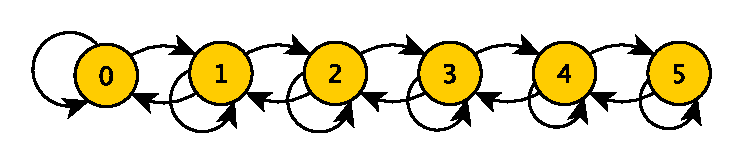
\includegraphics[width=\unitlength]{imgs/markowski.pdf}}
\small
\put(0,0.12){\rotatebox{90}{$1-\lambda\cdot\Delta t$}}
\put(0.17,0.28){$\lambda\cdot\Delta t$}
\put(0.10,0.10){\rotatebox{45}{$\mu\cdot\Delta t$}}
\put(0.33,0.28){$\lambda\cdot\Delta t$}
\put(0.29,0.09){\rotatebox{45}{$2\mu\cdot\Delta t$}}
\put(0.49,0.28){$\lambda\cdot\Delta t$}
\put(0.45,0.08){\rotatebox{45}{$3\mu\cdot\Delta t$}}
\put(0.65,0.28){$\lambda\cdot\Delta t$}
\put(0.60,0.08){\rotatebox{45}{$3\mu\cdot\Delta t$}}
\put(0.81,0.28){$\lambda\cdot\Delta t$}
\put(0.75,0.08){\rotatebox{45}{$3\mu\cdot\Delta t$}}
%\tiny
%\footnotesize
\scriptsize
\put(0.11,0.030){\rotatebox{45}{$1-(\mu+\lambda)\Delta t$}}
\put(0.27,0.016){\rotatebox{45}{$1-(2\mu+\lambda)\Delta t$}}
\put(0.44,0.014){\rotatebox{45}{$1-(3\mu+\lambda)\Delta t$}}
\put(0.59,0.020){\rotatebox{45}{$1-(3\mu+\lambda)\Delta t$}}
\put(0.74,0.020){\rotatebox{45}{$1-(3\mu+\lambda)\Delta t$}}
\Huge
\put(0.97,0.225){\ldots}
\normalsize
\end{picture}
\caption{Fronta THO jako markovský proces. Zákazníci přicházejí s paramtrem \(\lambda\) 
a můžou být obslouženi u jedné ze 3 přepážek. Doba obsluhy je popsána parametrem \(\mu\). 
Délka fronty jsou jednotlivé stavy markovského procesu. }
\label{fig:markowski}
\end{figure}
\end{frame}

\begin{frame}{Model s diskrétním časem}
\begin{itemize}
	\item čas simulace \(T\) na \(M\) poditervalů délky \(\Delta t\)
    \item \(\Delta t\) tak, že \(P[X\geq 2] \approx 0\)
    \item velmi jednoduchý, ale neefektivní
\end{itemize}
\end{frame}

\begin{frame}{Model s diskrétními událostmi}
\begin{figure}
\definecolor{ffqqqq}{rgb}{1.,0.,0.}
\definecolor{qqzzff}{rgb}{0.,0.6,1.}
\definecolor{qqqqff}{rgb}{0.,0.,1.}
\definecolor{cqcqcq}{rgb}{0.7529411764705882,0.7529411764705882,0.7529411764705882}
\begin{tikzpicture}[line cap=round,line join=round,>=triangle 45,x=0.3cm,y=0.8cm]
\draw [color=cqcqcq,, xstep=1.5cm,ystep=0.8cm] (0,-7.5) grid (32,0.5);
\draw[->,color=black] (-3.,0.) -- (32,0.);
\foreach \x in {,5.,10.,15.,20.,25.,30.}
\draw[shift={(\x,0)},color=black] (0pt,2pt) -- (0pt,-2pt) node[above] {\footnotesize $\x$};
\draw[<-,color=black] (0.,-7.5) -- (0.,0.5);
\foreach \y in {7.,6.,5.,4.,3.,2.,1.}
\draw[shift={(0,-\y)},color=black] (2pt,0pt) -- (-2pt,0pt) node[left] {\footnotesize $\y$};
\draw[color=black] (0pt,-10pt) node[right] {\footnotesize $0$};
\clip(-3.,-8.5) rectangle (46.010087437351785,0.507536612606849);
\draw [line width=4.pt,color=qqzzff] (1.8,-1.)-- (11.,-1);
\draw [line width=4.pt,color=qqzzff] (3.9,-2.)-- (13.,-2.);
\draw [line width=4.pt,color=qqzzff] (8.,-3.)-- (16.,-3.);
\draw [line width=3.2pt,color=ffqqqq] (9.2,-4.)-- (11.,-4.);
\draw [line width=4.pt,color=qqzzff] (15.,-5.)-- (22.,-5);
\draw [line width=4.pt,color=qqzzff] (11.,-4.)-- (20.,-4.);
\draw [line width=3.2pt,color=ffqqqq] (15.8,-6.)-- (20.,-6.);
\draw [line width=4.pt,color=qqzzff] (20.,-6.)-- (26.,-6.);
\draw [line width=3.2pt,color=ffqqqq] (18.,-7.)-- (22.,-7.);
\draw [line width=4.pt,color=qqzzff] (22.,-7.)-- (29.5,-7.);
\begin{scriptsize}
\draw [fill=qqqqff] (1.8,-1.) circle (2.5pt);
\draw[color=qqqqff] (2.4284789958647366,-0.6376375884262001) node {$A$};
\draw [fill=qqqqff] (3.9,-2.) circle (2.5pt);
\draw[color=qqqqff] (4.463417911420552,-1.644601110024226) node {$B$};
\draw [fill=qqqqff] (8.,-3.) circle (2.5pt);
\draw[color=qqqqff] (8.618084864013674,-2.6515646316222523) node {$C$};
\draw [fill=qqqqff] (9.2,-4.) circle (2.5pt);
\draw[color=qqqqff] (9.805132564754567,-3.6387837704438466) node {$D$};
\draw [fill=qqqqff] (15.,-5.) circle (2.5pt);
\draw[color=qqqqff] (15.570792825496044,-4.6457472920418725) node {$E$};
\draw [fill=qqqqff] (15.8,-6.) circle (2.5pt);
\draw[color=qqqqff] (16.418684040310968,-5.6527108136398985) node {$F$};
\draw [fill=qqqqff] (18.,-7.) circle (2.5pt);
\draw[color=qqqqff] (18.62320119882977,-6.639929952461492) node {$G$};
\end{scriptsize}
% casovy krok
\only<1>{\draw [line width=1.4pt,color=ffqqqq] (1.8,0.)-- (1.8,-7.5)};
\only<2>{\draw [line width=1.4pt,color=ffqqqq] (3.9,0.)-- (3.9,-7.5)};
\only<3>{\draw [line width=1.4pt,color=ffqqqq] (8,0.)-- (8,-7.5)};
\only<4>{\draw [line width=1.4pt,color=ffqqqq] (9,0.)-- (9,-7.5)};
\only<5>{\draw [line width=1.4pt,color=ffqqqq] (11,0.)-- (11,-7.5)};
\only<6>{\draw [line width=1.4pt,color=ffqqqq] (13,0.)-- (13,-7.5)};
\only<7>{\draw [line width=1.4pt,color=ffqqqq] (15,0.)-- (15,-7.5)};
\only<8>{\draw [line width=1.4pt,color=ffqqqq] (15.8,0.)-- (15.8,-7.5)};
\only<9>{\draw [line width=1.4pt,color=ffqqqq] (13,0.)-- (13,-7.5)};
\only<10>{\draw [line width=1.4pt,color=ffqqqq] (18,0.)-- (18,-7.5)};
\only<11>{\draw [line width=1.4pt,color=ffqqqq] (20,0.)-- (20,-7.5)};
\only<12>{\draw [line width=1.4pt,color=ffqqqq] (22,0.)-- (22,-7.5)};
\only<13>{\draw [line width=1.4pt,color=ffqqqq] (26,0.)-- (26,-7.5)};
\only<14>{\draw [line width=1.4pt,color=ffqqqq] (29.5,0.)-- (29.5,-7.5)};
\end{tikzpicture}
\end{figure}
\end{frame}

\begin{frame}{Ustálený stav}
\[\forall k \qquad p_k = \lim_{t\to\infty} p_k(t)\]
\(p_k\)\ldots počet zákazníků v pekárně
\begin{itemize}
	\item Nutná podmínka: \[\lambda < n\mu \]
\end{itemize}
\end{frame}
\begin{frame}{Ustálený stav}
\begin{figure}
\centering
\includegraphics[width=0.8\columnwidth]{imgs/fronta.pdf}
\label{fig:fronta}
\caption{Vývoj počtu zákazník ve frontě v průběhu 16 hodin. Fronta je bez omezení, vstupní tok \(\lambda = 100 \mbox{~h}^{-1}\). }
\end{figure}
\end{frame}